\chapter{Horizonte demográfico}

\marginal{la aportación del documento}
Este capítulo no existe en el género y es la razón por la que este documento se
escribió. Los tres rubros más grandes del presupuesto —pensiones, salud y
educación— son transferencias de ciclo de vida, y las tres se mueven con la
estructura de edades de la población. El paquete las presupuesta sin decir qué
supone sobre esa estructura.

\section{La tríada}

\begin{table}[htbp]
\centering
\caption{La tríada de cuentas de transferencias nacionales: los tres vértices}
\label{tab:C13_1}
\small
\begin{tabular}{lSSSp{3.2cm}p{4.2cm}}
\toprule
{Vértice} & {2025 (mdp)} & {\% PIB} & {Var. real \%} & {Dirección demográfica} & {¿Horizonte en el paquete?} \\
\midrule
{Pensiones contributivas (clasificacion economica)} & \num{1637665.1} & \num{4.53} & \num{4.7} & {la transicion lo empuja al alza} & {SI: el CGPE proyecta pensiones y jubilaciones a 2030 (4.5 a 4.8 \% del PIB)} \\
{Pensiones no contributivas (ramo 20)} & \num{527389.1} & \num{1.46} & \num{2.6} & {la transicion lo empuja al alza} & {NO: el paquete no proyecta el padron} \\
{Salud (funcion 2.3, GF + entidades, bruta)} & \num{888903.7} & \num{2.46} & \num{-12.2} & {al alza por envejecimiento} & {NO: ninguna proyeccion por funcion} \\
{Educacion (funcion 2.5, GF, bruta)} & \num{1084590.9} & \num{3.0} & \num{0.7} & {LA TRANSICION LO EMPUJA A LA BAJA} & {NO: el paquete no declara matricula, cobertura, planteles ni docentes} \\
\bottomrule
\end{tabular}
\par\vspace{2pt}\footnotesize Fuente: elaboración propia del ITED con los analíticos del PEF aprobado 2024 y 2025 y el CGPE 2025.
\end{table}


Los tres vértices con los mismos perímetros de sus capítulos, para que la
comparación no sea entre objetos distintos.

Las pensiones contributivas valen 4.53\% del PIB y crecen 4.7\% real. Las no
contributivas 1.46\% y crecen 2.6\%. La salud vale 2.46\% y cae 12.2\%, con la
descomposición del capítulo 6. La educación vale 3.00\% y crece 0.7\%.

\textbf{En conjunto, la tríada consume 11.45\% del PIB, casi la mitad del gasto
neto total.} Y su composición se desplaza de forma consistente: el vértice de la
vejez crece, el de la juventud se mantiene, el del ciclo completo cae.

\begin{figure}[htbp]
\centering
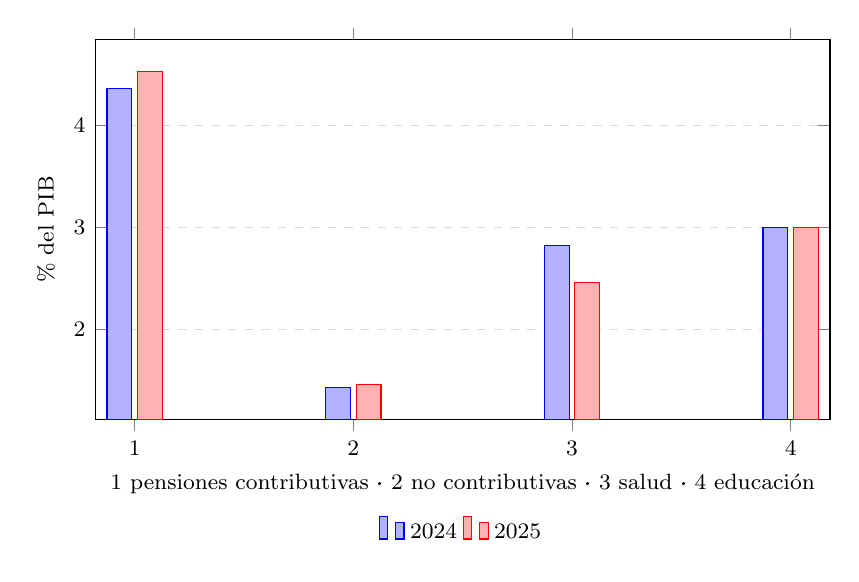
\begin{tikzpicture}
\begin{axis}[
  width=0.9\textwidth, height=6.4cm,
  xlabel={1 pensiones contributivas · 2 no contributivas · 3 salud · 4 educación}, ylabel={\% del PIB},
  legend style={font=\footnotesize, at={(0.5,-0.24)}, anchor=north,
                 legend columns=-1, draw=none},
  tick label style={font=\footnotesize},
  label style={font=\footnotesize},
  x tick label style={/pgf/number format/1000 sep={}},
  ymajorgrids=true, grid style={dashed, gray!30},
  enlarge x limits=0.06,
  cycle list={{solid,mark=*}, {dashed,mark=square*}, {dotted,mark=triangle*}, {dashdotted,mark=diamond*}},
  ybar, bar width=9pt,
  xtick=data,
]
\addplot+ coordinates {(1,4.36) (2,1.43) (3,2.82) (4,3.0)};
\addlegendentry{2024}
\addplot+ coordinates {(1,4.53) (2,1.46) (3,2.46) (4,3.0)};
\addlegendentry{2025}
\end{axis}
\end{tikzpicture}
\caption{La tríada de transferencias de ciclo de vida, 2024 y 2025}
\label{fig:F13_1}
\par\vspace{2pt}\footnotesize Fuente: elaboración propia del ITED con los analíticos del PEF aprobado 2024 y 2025. Mismos perímetros que los capítulos 5, 6 y 7.
\end{figure}


\section{Dónde declara el paquete un supuesto demográfico}

Se buscó pieza por pieza. El resultado es asimétrico y ésa es la tesis del
capítulo.

\begin{itemize}
\item \textbf{Pensiones: sí hay horizonte.} El CGPE proyecta pensiones y
jubilaciones de 4.5\% del PIB en 2025 a 4.8\% en 2030. Es la única función del
gasto con trayectoria publicada.
\item \textbf{Salud: no hay horizonte.} No hay proyección por función ni supuesto
de población por afiliación en ninguna pieza.
\item \textbf{Educación: no hay horizonte y tampoco denominador.} No hay
matrícula, cobertura, planteles ni docentes en el CGPE, la Ley de Ingresos o el
decreto.
\end{itemize}

\marginal{la matrícula se pide y no se usa}
La palabra matrícula aparece exactamente \textbf{dos veces} en el decreto de
Presupuesto de Egresos, y las dos son obligaciones de reportarla: las
instituciones públicas de educación superior deben auditar su matrícula
externamente y enviar los resultados, y debe informarse la matrícula de inicio y
fin de cada ciclo escolar.

\textbf{El paquete obliga a producir la cifra y no asigna un solo peso con ella.}
La información existe, se recoge por mandato legal, y no entra en la decisión
presupuestaria ni en su justificación pública.

\section{La asimetría}

\textbf{El paquete tiene horizonte demográfico donde la demografía presiona al
alza y no lo tiene donde presiona a la baja.}

Pensiones es el rubro donde la transición encarece el compromiso año con año, y es
el único con proyección. Educación es el rubro donde la población en edad escolar
se contrae, de modo que un gasto plano en términos reales mejora por alumno sin
que nadie decida nada, y es el rubro sin una sola cifra de población.

La asimetría tiene una consecuencia práctica que conviene enunciar sin
dramatismo: \textbf{el paquete puede sostener que mantiene el gasto educativo y
puede estar, al mismo tiempo, aumentándolo o reduciéndolo por alumno, y nadie
puede saber cuál con las piezas publicadas.} La proyección de pensiones, en
cambio, permite discutir. Discutir requiere denominadores, y el paquete publica
uno de tres.

\section{Lo que este capítulo no afirma}

No se afirma que el gasto educativo por alumno haya subido o bajado. \textbf{No se
puede saber} y ése es precisamente el punto. Tampoco se afirma que la proyección
de pensiones sea correcta: tres décimas de punto del PIB en seis años es una
trayectoria notablemente plana para una población que envejece, y el paquete no
publica el supuesto que la sostiene, de modo que no es verificable.

Lo que sí se afirma, y se sostiene con la búsqueda documentada arriba, es que
\textbf{de los tres vértices de la tríada, dos carecen de denominador publicado y
uno tiene una proyección sin supuesto declarado.}

\clearpage
